\section*{7. \"Ubung (Abgabe: 16.06.2010, 8.30 Uhr, schriftlich)}

\subsection*{1.a. Wie stark muss man ein n-dimensionales Signal gl\"atten, um die Standardabweichung des Rauschens zu halbieren?}

\begin{align*}
Gegeben:\; \sigma_{reduced\;noise}^{2} &\approx \frac{1}{(2\sqrt{\pi}\sigma_{Gauss})^{n}} \sigma_{noise}^{2} \\
Ansatz:\; \sigma_{reduced\; noise} &:= \frac{1}{2}\sigma_{noise} \\
(\frac{1}{2}\sigma_{noise})^{2} &\approx \frac{1}{(2\sqrt{\pi}\sigma_{Gauss})^{n}} \sigma_{noise}^{2} \\
\frac{1}{2}\sigma_{noise} &\approx \frac{1}{(2\sqrt{\pi}\sigma_{Gauss})^{\frac{n}{2}}} \sigma_{noise},\; \sigma_{noise}>0 \\
\frac{1}{2} &\approx \frac{1}{(2\sqrt{\pi}\sigma_{Gauss})^{\frac{n}{2}}} \\
2 &\approx (2\sqrt{\pi}\sigma_{Gauss})^{\frac{n}{2}} \\
4 &\approx (2\sqrt{\pi}\sigma_{Gauss})^{n} \\
\sqrt[n]{4} &\approx 2\sqrt{\pi}\sigma_{Gauss} \\
\sqrt[n]{4}\cdot\frac{1}{2\sqrt{\pi}} &\approx \sigma_{Gauss} \\
\end{align*}
Das bedeutet, je mehr Dimensionen das Eingangssignal hat, desto geringer muss die Gl\"attung ausfallen, um die Standardabweichung des Rauschens zu halbieren.

\begin{figure}[!h] %  figure placement: here, top, bottom, or page
   \centering
   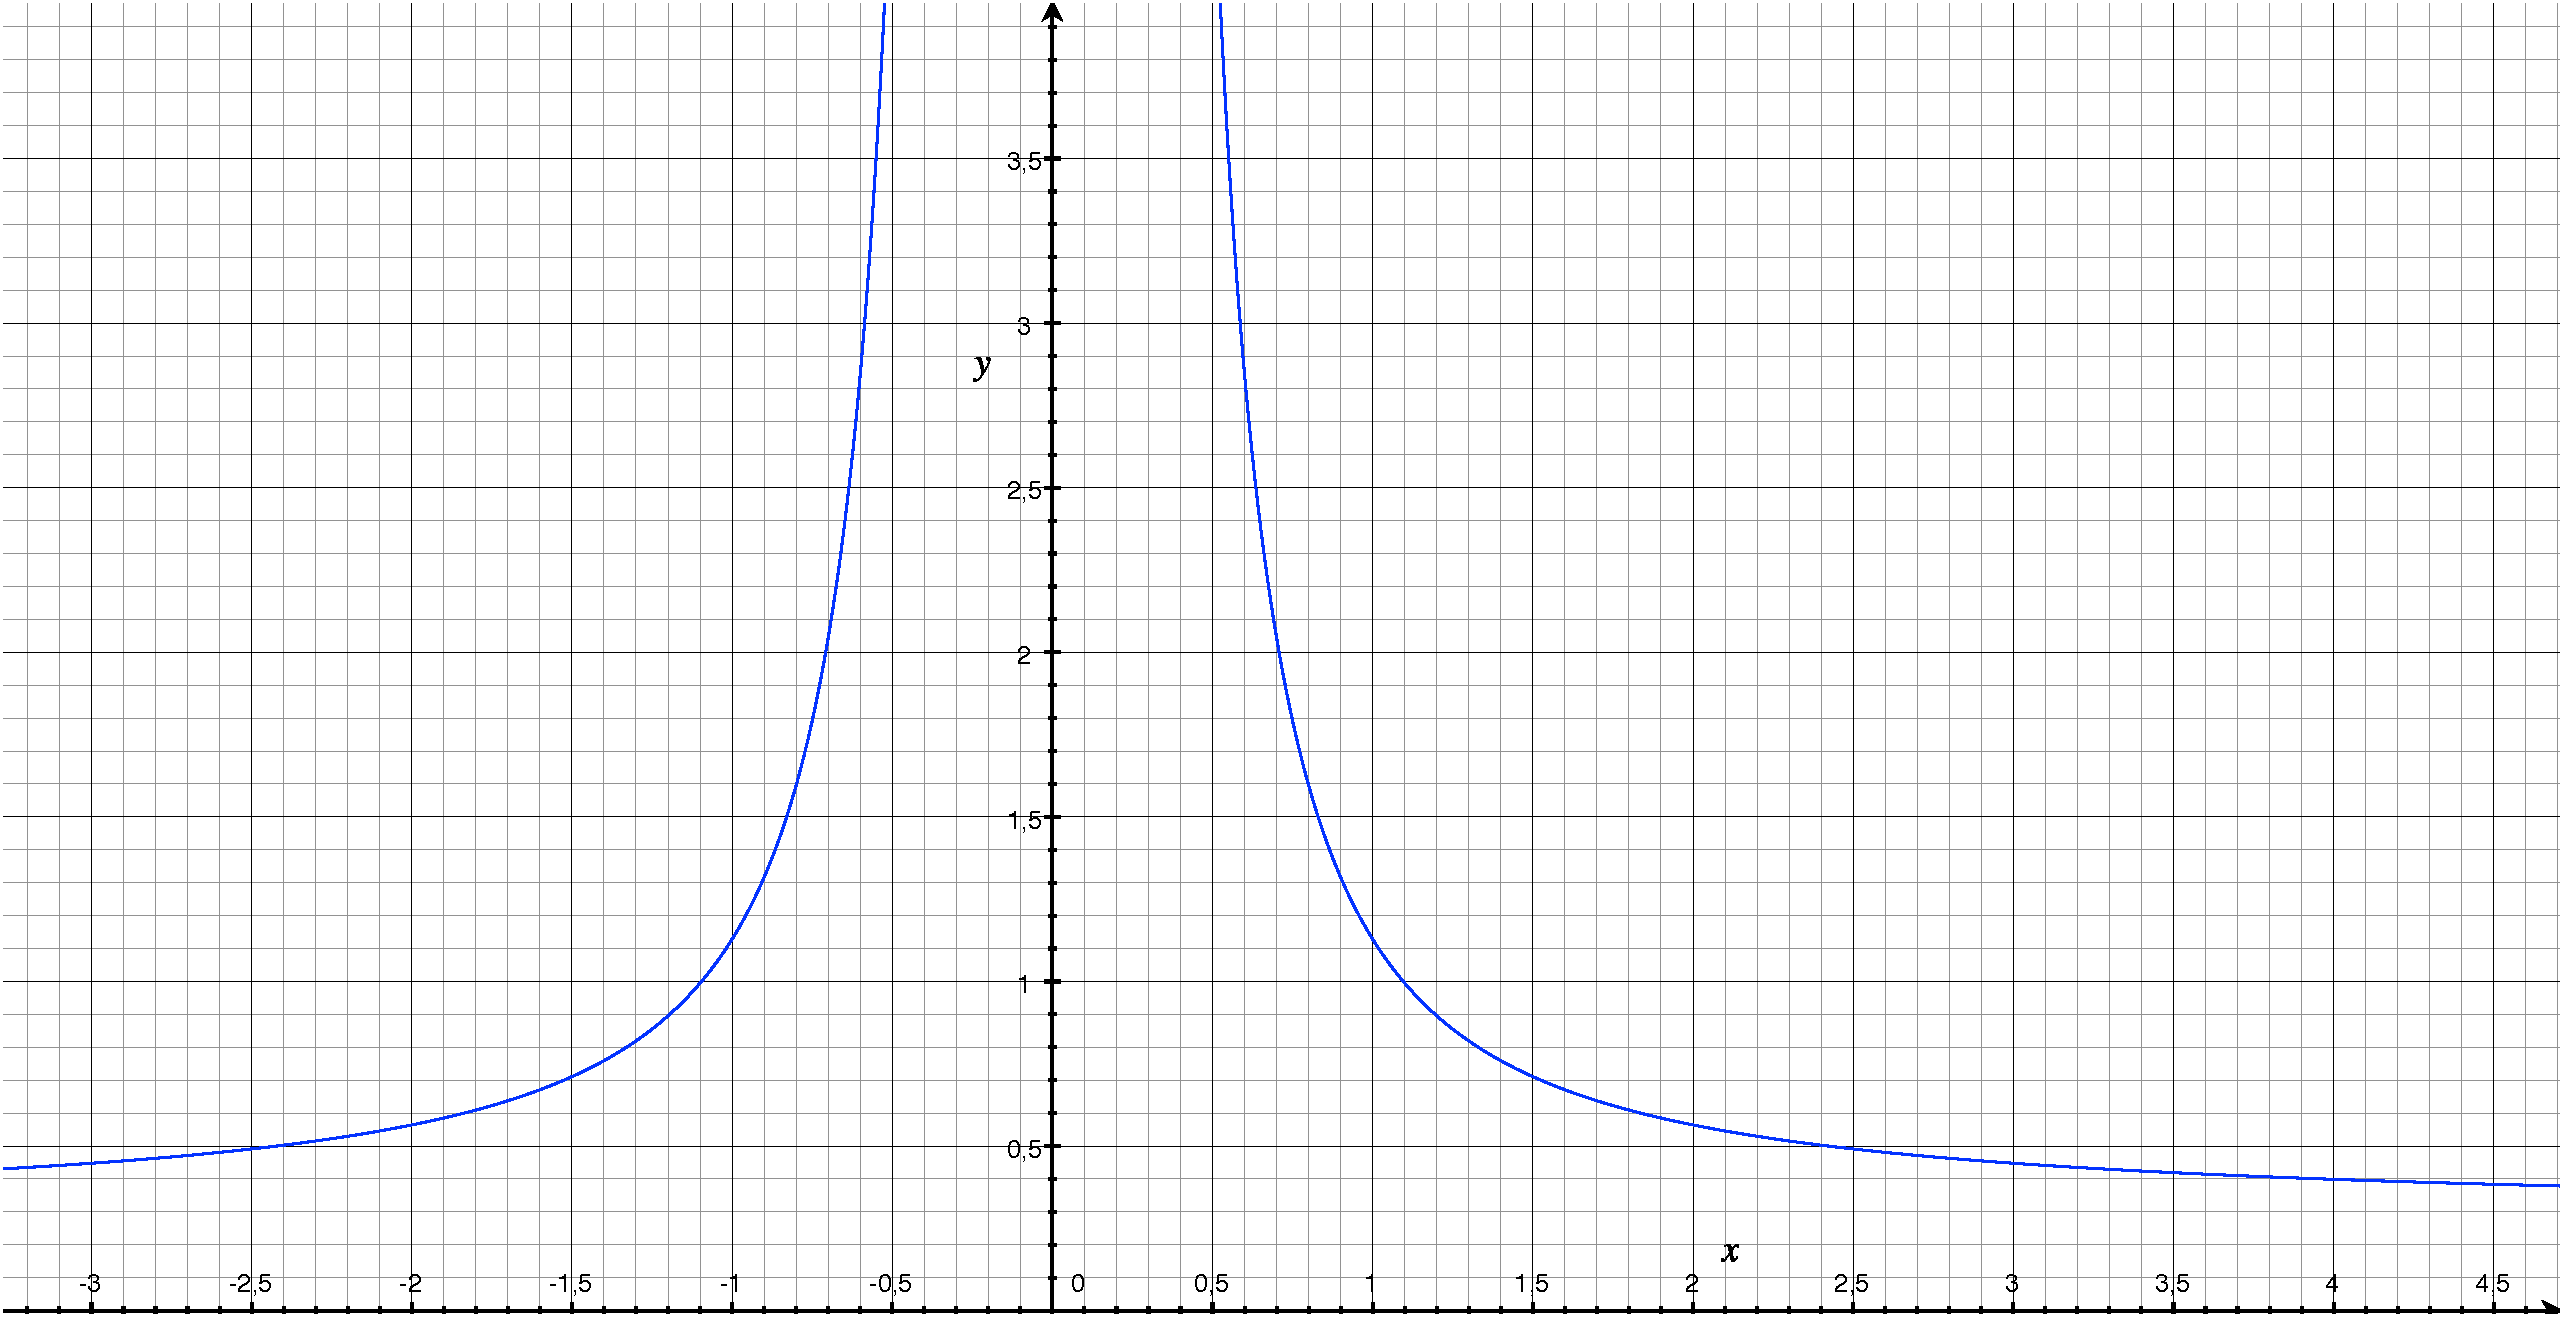
\includegraphics[height=0.17\textheight]{Uebung7/1_a.pdf} 
   \caption{Zusammenhang von Dimension (x$=\mid n \mid$) und Gl\"attung (y$=\sigma_{Gauss}$)}
   \label{fig:5.1}
\end{figure}

\subsection*{1.b. Auf welche Weise h\"angt die Varianz des Lokalisierungsfehlers f\"ur die F\"alle n=1,2,3 von dem Grad des urspr\"unglichen Rauschens und dem Grad der Gl\"attung ab? Was bedeutet das f\"ur die Anwendung von schwellenwertbasierten Kantendetektoren in verrauschten zweidimensionalen Bildern?}
